\documentclass[14pt,a4paper]{extarticle}
% =============================================================
% preamble.tex — оформление отчётов по СТП БГУИР 01-2024
% =============================================================

% Шрифты: под pdflatex — Times через tempora + T2A,
% под xelatex/tectonic — системный Times New Roman (запасной вариант STIX Two Text)
\usepackage{iftex}
\ifPDFTeX
  \usepackage[utf8]{inputenc}
  \usepackage[T2A]{fontenc}
  \usepackage{tempora}
\else
  \usepackage{fontspec}
  \IfFontExistsTF{Times New Roman}
    {\setmainfont{Times New Roman}}
    {\setmainfont{STIX Two Text}}
  \IfFontExistsTF{DejaVu Sans Mono}
    {\setmonofont{DejaVu Sans Mono}[Scale=0.82]}
    {\setmonofont{DejaVuSansMono}[Extension=.ttf, BoldFont=*-Bold,
                                  ItalicFont=*-Oblique, Scale=0.82]}
\fi
\usepackage[russian]{babel}

% Поля: слева 30 мм, справа 15 мм, сверху и снизу 20 мм
\usepackage{geometry}
\geometry{left=30mm, right=15mm, top=20mm, bottom=20mm}

\usepackage{setspace}
\singlespacing

\pretolerance=1000
\tolerance=2000
\emergencystretch=3em

\usepackage{indentfirst}
\setlength{\parindent}{1.25cm}

% Номер страницы — снизу справа
\usepackage{fancyhdr}
\pagestyle{fancy}
\fancyhf{}
\fancyfoot[R]{\thepage}
\renewcommand{\headrulewidth}{0pt}
\fancypagestyle{plain}{%
  \fancyhf{}%
  \fancyfoot[R]{\thepage}%
  \renewcommand{\headrulewidth}{0pt}%
}

\usepackage{amsmath,amssymb}
\usepackage{graphicx}
\usepackage{float}
\usepackage{booktabs}
\usepackage{tabularx}
\usepackage{multirow}
\usepackage{longtable}
\usepackage{array}

\usepackage{caption}
\captionsetup[figure]{labelsep=endash, justification=centering,
                      font={normalsize}, name=Рисунок}
\captionsetup[table]{labelsep=endash, justification=raggedright,
                     singlelinecheck=false, font={normalsize}, name=Таблица}

\usepackage{titlesec}
\titleformat{\section}
  {\normalfont\fontsize{14}{18}\selectfont\bfseries}
  {\thesection}{0.5em}{\MakeUppercase}
\titlespacing*{\section}{1.25cm}{0pt}{14pt}
% Разрыв страницы до заголовка, чтобы номер в содержании совпадал со страницей раздела
\newcommand{\sectionbreak}{\clearpage}
\titleformat{\subsection}
  {\normalfont\fontsize{14}{18}\selectfont\bfseries}
  {\thesubsection}{0.5em}{}
\titlespacing*{\subsection}{1.25cm}{14pt}{14pt}
\titleformat{\subsubsection}
  {\normalfont\fontsize{14}{18}\selectfont\bfseries}
  {\thesubsubsection}{0.5em}{}
\titlespacing*{\subsubsection}{1.25cm}{14pt}{14pt}

\newcommand{\sectioncenter}[1]{%
  \newpage
  \phantomsection
  \addcontentsline{toc}{section}{#1}
  \begin{center}\textbf{\MakeUppercase{#1}}\end{center}
  \vspace{14pt}
}

\usepackage{tocloft}
\renewcommand{\cftsecfont}{\normalfont}
\renewcommand{\cftsecpagefont}{\normalfont}
\renewcommand{\cftsubsecfont}{\normalfont}
\renewcommand{\cftsubsecpagefont}{\normalfont}
\renewcommand{\cftsecleader}{\cftdotfill{\cftdotsep}}
\renewcommand{\cftdotsep}{1}
% babel переопределяет заголовки после преамбулы, поэтому правим через \addto
\addto\captionsrussian{\renewcommand{\contentsname}{\hfill\textbf{СОДЕРЖАНИЕ}\hfill}}
\renewcommand{\cftaftertoctitle}{\hfill}

\usepackage{enumitem}
\setlist[itemize]{noitemsep, topsep=0pt, leftmargin=1.25cm, label=--}
\setlist[enumerate]{noitemsep, topsep=0pt, leftmargin=1.25cm}

% Листинги кода и вывода программы
\usepackage{listings}
\usepackage{fancyvrb}
\lstset{
  basicstyle=\ttfamily\footnotesize,
  frame=single,
  breaklines=true,
  showstringspaces=false,
  inputencoding=utf8,
  extendedchars=true,
  columns=fullflexible,
  keepspaces=true,
  captionpos=t
}
\ifPDFTeX
\lstset{
  literate={а}{{\cyra}}1 {б}{{\cyrb}}1 {в}{{\cyrv}}1 {г}{{\cyrg}}1
           {д}{{\cyrd}}1 {е}{{\cyre}}1 {ж}{{\cyrzh}}1 {з}{{\cyrz}}1
           {и}{{\cyri}}1 {й}{{\cyrishrt}}1 {к}{{\cyrk}}1 {л}{{\cyrl}}1
           {м}{{\cyrm}}1 {н}{{\cyrn}}1 {о}{{\cyro}}1 {п}{{\cyrp}}1
           {р}{{\cyrr}}1 {с}{{\cyrs}}1 {т}{{\cyrt}}1 {у}{{\cyru}}1
           {ф}{{\cyrf}}1 {х}{{\cyrh}}1 {ц}{{\cyrc}}1 {ч}{{\cyrch}}1
           {ш}{{\cyrsh}}1 {щ}{{\cyrshch}}1 {ъ}{{\cyrhrdsn}}1
           {ы}{{\cyrery}}1 {ь}{{\cyrsftsn}}1 {э}{{\cyrerev}}1
           {ю}{{\cyryu}}1 {я}{{\cyrya}}1 {ё}{{\cyryo}}1
           {А}{{\CYRA}}1 {Б}{{\CYRB}}1 {В}{{\CYRV}}1 {Г}{{\CYRG}}1
           {Д}{{\CYRD}}1 {Е}{{\CYRE}}1 {Ж}{{\CYRZH}}1 {З}{{\CYRZ}}1
           {И}{{\CYRI}}1 {Й}{{\CYRISHRT}}1 {К}{{\CYRK}}1 {Л}{{\CYRL}}1
           {М}{{\CYRM}}1 {Н}{{\CYRN}}1 {О}{{\CYRO}}1 {П}{{\CYRP}}1
           {Р}{{\CYRR}}1 {С}{{\CYRS}}1 {Т}{{\CYRT}}1 {У}{{\CYRU}}1
           {Ф}{{\CYRF}}1 {Х}{{\CYRH}}1 {Ц}{{\CYRC}}1 {Ч}{{\CYRCH}}1
           {Ш}{{\CYRSH}}1 {Щ}{{\CYRSHCH}}1 {Ъ}{{\CYRHRDSN}}1
           {Ы}{{\CYRERY}}1 {Ь}{{\CYRSFTSN}}1 {Э}{{\CYREREV}}1
           {Ю}{{\CYRYU}}1 {Я}{{\CYRYA}}1 {Ё}{{\CYRYO}}1
           {—}{{---}}1 {–}{{--}}1 {…}{{\ldots}}1
}
\fi

% Подписи листингов — в том же стиле, что таблицы: «Листинг X.Y — Название»
\captionsetup[lstlisting]{labelsep=endash, justification=raggedright,
                          singlelinecheck=false, font={normalsize}}
\renewcommand{\lstlistingname}{Листинг}
\AtBeginDocument{\numberwithin{lstlisting}{section}}

\lstdefinestyle{python}{language=Python, keywordstyle=\bfseries}
\lstdefinestyle{shell}{language=bash, keywordstyle=\mdseries}
\lstdefinestyle{plain}{language={}, basicstyle=\ttfamily\scriptsize}

% Абзац после листинга должен сохранять отступ 1,25 см (СТП 2.1.1)
\makeatletter
\AtBeginDocument{\let\@endpetrue\@endpefalse}
\makeatother

% Подпись к блоку verbatim: \captionof вне плавающего окружения
% глобально обнуляет \parindent, поэтому отступ восстанавливается вручную
\newcommand{\listingcaption}[2]{%
  \captionof{lstlisting}{#1}\label{#2}%
  \setlength{\parindent}{1.25cm}%
}

\usepackage{hyperref}
\hypersetup{colorlinks=true, linkcolor=black, urlcolor=blue, citecolor=black}

\numberwithin{figure}{section}
\numberwithin{table}{section}
\numberwithin{equation}{section}

% Титульный лист отчёта по лабораторной работе
\newcommand{\makelabtitle}[2]{%
  \begin{titlepage}
  \thispagestyle{empty}
  \begin{center}

  МИНИСТЕРСТВО ОБРАЗОВАНИЯ РЕСПУБЛИКИ БЕЛАРУСЬ

  \vspace{0.5em}
  Учреждение образования

  \vspace{0.5em}
  \textbf{<<Белорусский государственный университет информатики и радиоэлектроники>>}

  \vspace{2em}
  Факультет компьютерных систем и сетей

  \vspace{0.5em}
  Кафедра программного обеспечения информационных технологий
  \end{center}

  \vspace{3em}
  \begin{center}
  \textbf{ОТЧЕТ}

  \vspace{0.5em}
  по лабораторной работе №#1

  \vspace{0.5em}
  по дисциплине

  \vspace{0.5em}
  <<Технологии компонентного программирования>>

  \vspace{0.5em}
  <<#2>>
  \end{center}

  \vspace{5em}
  \begin{flushright}
  \begin{minipage}{0.5\textwidth}
  \textbf{Выполнил:}\\
  Лебедевич Артем Владимирович\\
  магистрант группы 556301

  \vspace{0.6em}
  \textbf{Преподаватель:}\\
  Герман Олег Витольдович\\
  кандидат технических наук\\
  доцент кафедры ИТАС
  \end{minipage}
  \end{flushright}

  \vfill
  \begin{center}Минск, 2026~г.\end{center}
  \end{titlepage}
}


\newcolumntype{L}{>{\raggedright\arraybackslash}X}

\begin{document}

\makelabtitle{3}{Brython: клиентский сайт на Python}

\tableofcontents

\section{Цель работы}

Изучить возможности фреймворка Brython, позволяющего писать клиентские сценарии
интернет-приложений на языке Python. Создать клиентский сайт, который находит корни
многочлена, строит прогноз с помощью линейной регрессии и находит оптимальное значение
функции без ограничений.

\section{Теоретические сведения}

\subsection{Brython}

Браузер выполняет только JavaScript. Brython --- это программа на JavaScript
(\texttt{brython.js}), которая находит на странице блоки
\texttt{<script type="text/python">}, переводит исходный текст на Python в JavaScript
прямо в браузере и выполняет его. Благодаря пакету \texttt{browser} программа получает
доступ к объектам DOM, поэтому обработчики событий, разметка и рисование на холсте
пишутся на Python. Основные понятия приведены в таблице~\ref{tab:terms}.

\begin{table}[H]
\caption{Основные понятия Brython}
\label{tab:terms}
\centering
\begin{tabularx}{\textwidth}{lL}
\toprule
Понятие & Смысл \\
\midrule
\texttt{brython.js} & компилятор и среда выполнения, подключаются тегом
\texttt{<script src>} \\
\texttt{brython\_stdlib.js} & стандартная библиотека Python в виде одного файла \\
\texttt{brython()} & функция, которая находит и запускает сценарии Python; вызывается
из \texttt{<body onload>} \\
\texttt{browser.document} & документ DOM: \texttt{document["id"]} --- элемент,
\texttt{elt.bind("click", f)} --- обработчик события \\
\texttt{browser.html} & конструкторы тегов: \texttt{html.H2("текст")};
\texttt{document <= элемент} добавляет элемент на страницу \\
\texttt{pythonpath} & каталоги, где \texttt{import} ищет собственные модули (они
загружаются запросом XHR) \\
\bottomrule
\end{tabularx}
\end{table}

Методические материалы рекомендуют не подключать Brython из облака, а использовать
локальную установку. Команда \texttt{pip install brython} копирует файлы
\texttt{brython.js} и \texttt{brython\_stdlib.js} в каталог пакета; скрипт
\texttt{scripts/fetch\_runtimes.py} переносит их в каталог сайта.

\subsection{Различия версий}

Методичка написана для Brython 3.9, в работе использована версия 3.15.0. При переходе
обнаружились три отличия, которые влияют на программу.

\begin{itemize}
\item Инструкция \texttt{import browser} больше не делает доступным
\texttt{browser.html}: нужно писать \texttt{import browser.html} или
\texttt{from browser import html}.
\item Brython кэширует стандартную библиотеку в IndexedDB. Браузер без окна, который
снимает DOM сразу после события \texttt{load}, видит недостроенную страницу; параметр
\texttt{brython(\{indexedDB: false\})} делает запуск последовательным.
\item Форматирование \texttt{"\%g" \% x} неверно для очень малых и очень больших чисел
(\texttt{2.2e-16} превращается в \texttt{0e+00}), тогда как
\texttt{"\{:g\}".format(x)} работает правильно. Поэтому сайт форматирует числа методом
\texttt{format}.
\end{itemize}

\subsection{Корни многочлена}

Для многочлена $p(x)=a_0x^n+\dots+a_n$ все корни, в том числе комплексные, находятся
методом Дурана --- Кернера. После деления на старший коэффициент берётся $n$ начальных
приближений на окружности, и каждое пересчитывается по формуле
\[
z_i \leftarrow z_i-\frac{p(z_i)}{\prod_{j\ne i}(z_i-z_j)} .
\]
Итерации прекращаются, когда наибольшая поправка меньше $10^{-14}$. Затем корни
уточняются несколькими шагами Ньютона по исходному многочлену. Многочлены первой и
второй степени решаются по формулам (для второй степени --- в устойчивой форме, без
вычитания близких чисел), нулевые последние коэффициенты дают точные нулевые корни.
Малые мнимые части (порядка $10^{-9}$) считаются вычислительным шумом и отбрасываются.

\subsection{Линейная регрессия}

По точкам $(x_i,y_i)$ строится прямая $y=ax+b$ методом наименьших квадратов:
\[
a=\frac{\sum (x_i-\bar x)(y_i-\bar y)}{\sum (x_i-\bar x)^2},\qquad b=\bar y-a\bar x .
\]
Качество оценивается коэффициентом детерминации $R^2=1-\sum e_i^2/\sum(y_i-\bar y)^2$ и
среднеквадратичной ошибкой. Прогноз --- значение прямой в следующих точках с шагом,
равным среднему расстоянию между исходными $x$. Для каждой точки прогноза строится
приближённая 95\,\% полоса
$\pm 1{,}96\,s\sqrt{1+1/n+(x_0-\bar x)^2/\sum(x_i-\bar x)^2}$, где $s$ --- остаточное
стандартное отклонение.

\subsection{Оптимум функции без ограничений}

Реализованы три метода.

\begin{itemize}
\item \textbf{Метод Нелдера --- Мида} (симплекс) не требует производных: из $n+1$
вершин заменяется худшая --- отражением, растяжением или сжатием, при неудаче весь
симплекс сжимается к лучшей вершине. Метод проходит узкую долину функции Розенброка.
\item \textbf{Градиентный спуск} движется против градиента, который вычисляется
центральными разностями; шаг подбирается делением пополам, пока не выполнится условие
Армихо $f(x-t\nabla f)\le f(x)-10^{-4}t\|\nabla f\|^2$.
\item \textbf{Золотое сечение} находит минимум унимодальной функции одной переменной
на заданном отрезке; отрезок сужается в $(\sqrt5-1)/2$ раз за шаг.
\end{itemize}

Максимум ищется как минимум функции $-f$. Функция вводится текстом (знак \texttt{\^{}}
означает степень), текст один раз компилируется в \texttt{lambda}, которой видны только
имена из модуля \texttt{math}; любое другое имя вызывает ошибку.

\section{Реализация}

\subsection{Структура программы}

\listingcaption{Структура лабораторной работы}{lst:tree}
\begin{Verbatim}[fontsize=\scriptsize, frame=single, samepage=true]
lab3/numerics.py           численные методы, только math и cmath
lab3/site/index.html       страница: три вкладки, поля ввода, холсты
lab3/site/app.py           код страницы на Python (запускается Brython)
lab3/site/examples.html    примеры из методички
lab3/site/brython*.js      Brython 3.15.0 (копируется скриптом)
lab3/server.py             HTTP-сервер каталога lab3/
lab3/cases.py              проверяемые сценарии
lab3/runner.py             запуск сценариев из командной строки
lab3/gui.py                окно: страница в WebView и список сценариев
\end{Verbatim}

Главная особенность решения: файл \texttt{numerics.py} один. Сервер отдаёт его браузеру
по адресу \texttt{/numerics.py}, страница подключает его инструкцией \texttt{import
numerics} (параметр \texttt{pythonpath: ['/']}), а тесты в CPython импортируют тот же
файл.

\subsection{Страница}

Разметка содержит заголовок, три кнопки вкладок и три раздела. Brython подключается в
конце страницы, а запускается по событию загрузки (листинг~\ref{lst:page}).

\begin{lstlisting}[style=plain, caption={Подключение Brython}, label={lst:page}]
<body onload="brython({pythonpath: ['/'], indexedDB: false})">
  ...
  <script src="brython.js"></script>
  <script src="brython_stdlib.js"></script>
  <script type="text/python" src="app.py"></script>
</body>
\end{lstlisting}

\subsection{Корни многочлена}

Обработчик кнопки читает коэффициенты, вызывает \texttt{poly\_roots} и строит таблицу
средствами \texttt{browser.html} (листинг~\ref{lst:roots}); корни отмечаются точками на
комплексной плоскости.

\begin{lstlisting}[style=python, caption={Обработчик вкладки корней}, label={lst:roots}]
def run_roots(ev=None):
    box = document["roots_result"]
    try:
        coeffs = nm.poly_trim(nm.parse_numbers(document["roots_coeffs"].value))
        roots = nm.poly_roots(coeffs)
    except ValueError as exc:
        show_error(box, str(exc))
        return
    box.clear()
    box <= html.DIV("p(x) = " + nm.poly_text(coeffs), Class="big")
    rows = [[str(i + 1), nm.root_text(r), "{:.2e}".format(abs(nm.poly_eval(coeffs, r)))]
            for i, r in enumerate(roots)]
    box <= table(["#", "root", "|p(root)|"], rows)
\end{lstlisting}

Основная часть метода Дурана --- Кернера (листинг~\ref{lst:dk}) --- обычный цикл по
комплексным числам, встроенный тип \texttt{complex} поддерживается Brython.

\begin{lstlisting}[style=python, caption={Метод Дурана --- Кернера}, label={lst:dk}]
monic = [c / coeffs[0] for c in coeffs]
radius = _cauchy_bound(monic)
guess = [radius * 0.5 * cmath.exp(2j * math.pi * k / degree + 0.4j) for k in range(degree)]
for _ in range(max_iter):
    largest = 0.0
    for i in range(degree):
        denominator = 1
        for j in range(degree):
            if i != j:
                denominator *= guess[i] - guess[j]
        step = poly_eval(monic, guess[i]) / denominator
        guess[i] -= step
        largest = max(largest, abs(step))
    if largest < tol:
        break
\end{lstlisting}

\subsection{Линейная регрессия}

Наблюдения вводятся строками \texttt{x y}; строка с одним числом задаёт ряд
$y(1),y(2),\dots$ Функция \texttt{linear\_regression} возвращает коэффициенты и
показатели качества, \texttt{forecast} продолжает ряд (листинг~\ref{lst:reg}).

\begin{lstlisting}[style=python, caption={Регрессия и прогноз}, label={lst:reg}]
def linear_regression(xs, ys):
    n = len(xs)
    mean_x, mean_y = sum(xs) / n, sum(ys) / n
    sxx = sum((x - mean_x) ** 2 for x in xs)
    sxy = sum((x - mean_x) * (y - mean_y) for x, y in zip(xs, ys))
    slope = sxy / sxx
    intercept = mean_y - slope * mean_x
    ...

def forecast(model, xs, steps):
    step = (xs[-1] - xs[0]) / (len(xs) - 1) if len(xs) > 1 else 1.0
    future = [xs[-1] + step * (k + 1) for k in range(int(steps))]
    return [(x, predict(model, x)) for x in future]
\end{lstlisting}

\subsection{Оптимум}

Функция из текстового поля превращается в обычную функцию один раз, поэтому
оптимизатор вызывает её без повторной компиляции (листинг~\ref{lst:compile}). Это
существенно для Brython: компиляция строки при каждом из сотен тысяч вызовов
градиентного спуска заняла бы минуты.

\begin{lstlisting}[style=python, caption={Компиляция введённой функции}, label={lst:compile}]
def compile_function(expression, dimension):
    source = expression.strip().replace("^", "**")
    names = VARIABLES[:dimension]
    for name in _identifiers(source):
        if name not in _SAFE and name not in names:
            raise ValueError("unknown name: " + name)
    scope = dict(_SAFE)
    scope["__builtins__"] = {}
    func = eval("lambda " + ", ".join(names) + ": (" + source + ")", scope)

    def f(point):
        return float(func(*point))
    return f
\end{lstlisting}

Для функции двух переменных страница строит тепловую карту (значения берутся по
логарифмической шкале) и рисует траекторию поиска, для функции одной переменной ---
график с точками траектории.

\subsection{Окно и сервер}

Класс \texttt{SiteServer} (модуль \texttt{lab3/server.py}) --- встроенный
\texttt{http.server} с корнем в каталоге \texttt{lab3/}: страницы лежат в
\texttt{/site/}, общий модуль --- в корне. Окно \texttt{python main.py -{}-lab 3
-{}-gui} показывает сайт в элементе WebView, кнопки открывают вкладки, справа находится
список проверок.

\section{Результаты работы программы}

На рисунке~\ref{fig:window} показано окно: слева сайт со вкладкой корней многочлена
$x^3-6x^2+11x-6$, справа --- шесть сценариев, все выполнены успешно.

\begin{figure}[H]
\centering
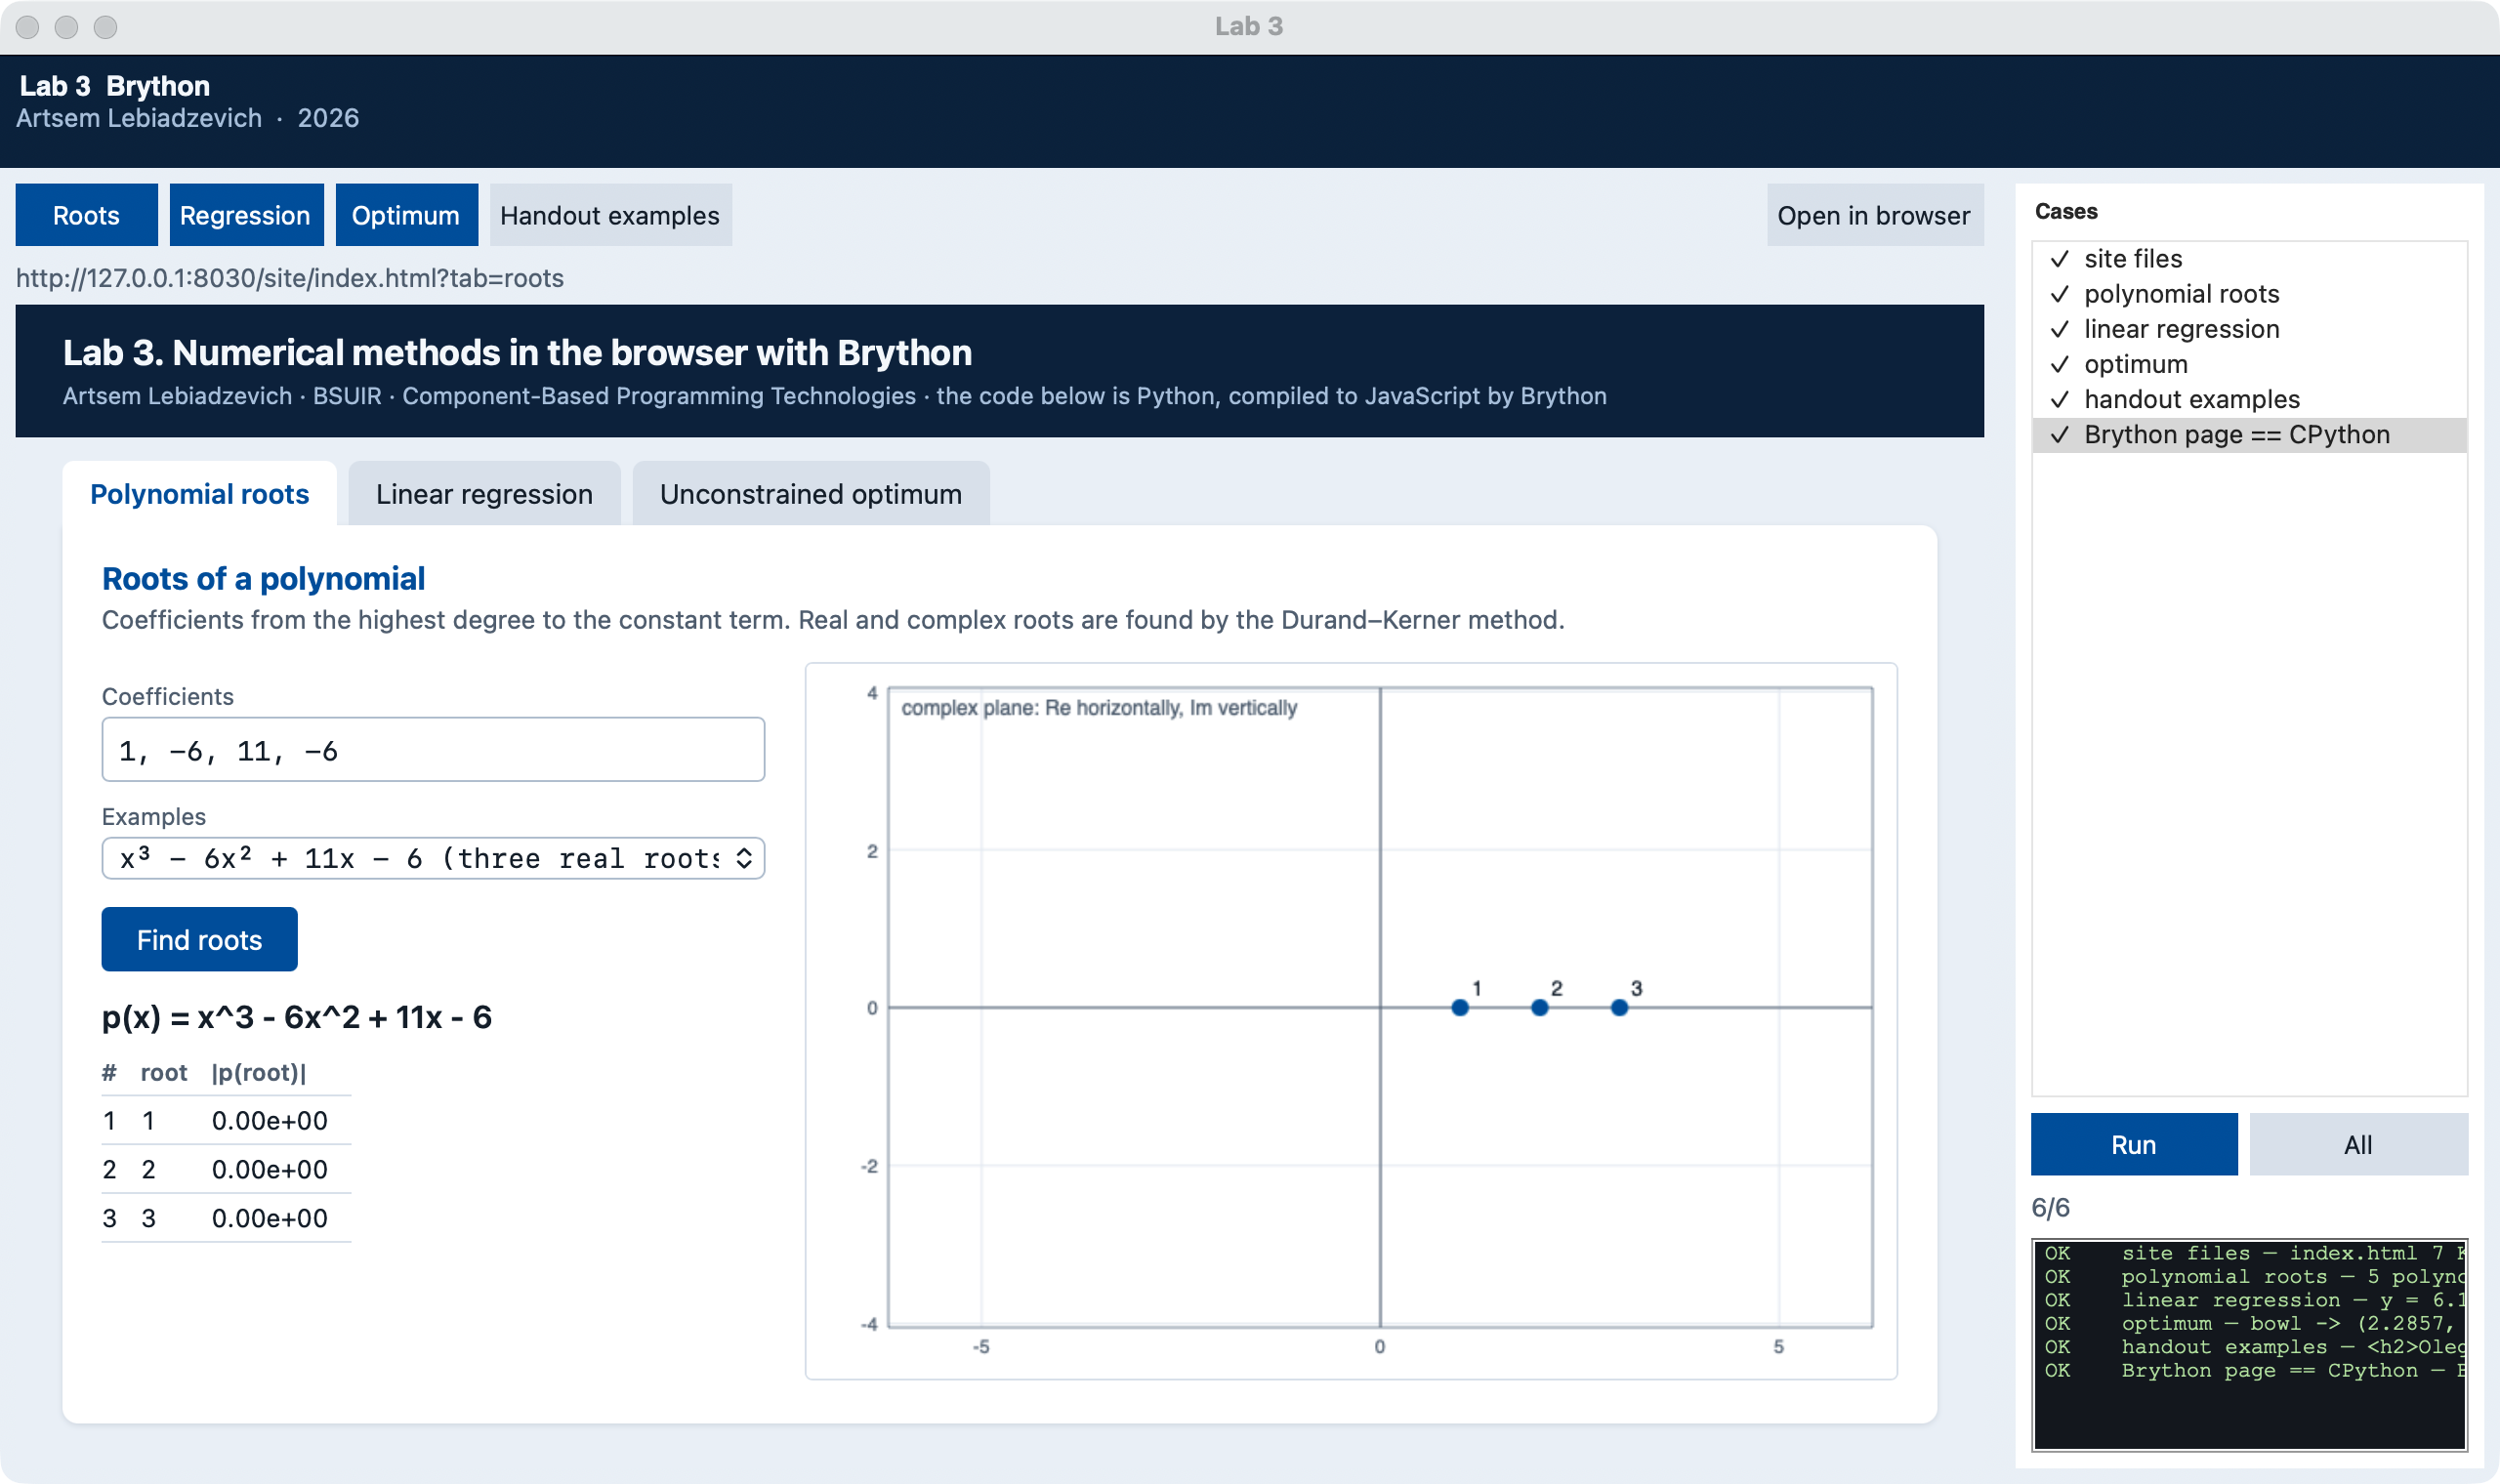
\includegraphics[width=0.95\textwidth]{../screenshots/lab3.png}
\caption{Окно лабораторной работы: сайт Brython и список проверок}
\label{fig:window}
\end{figure}

Вкладка регрессии (рисунок~\ref{fig:reg}) показывает десять наблюдений, прямую
$y=6{,}139x+95{,}33$ ($R^2=0{,}995$) и прогноз на четыре шага вперёд и в точке $x=20$;
оранжевая полоса --- приближённый 95\,\% интервал, он расширяется по мере удаления от
данных.

\begin{figure}[H]
\centering
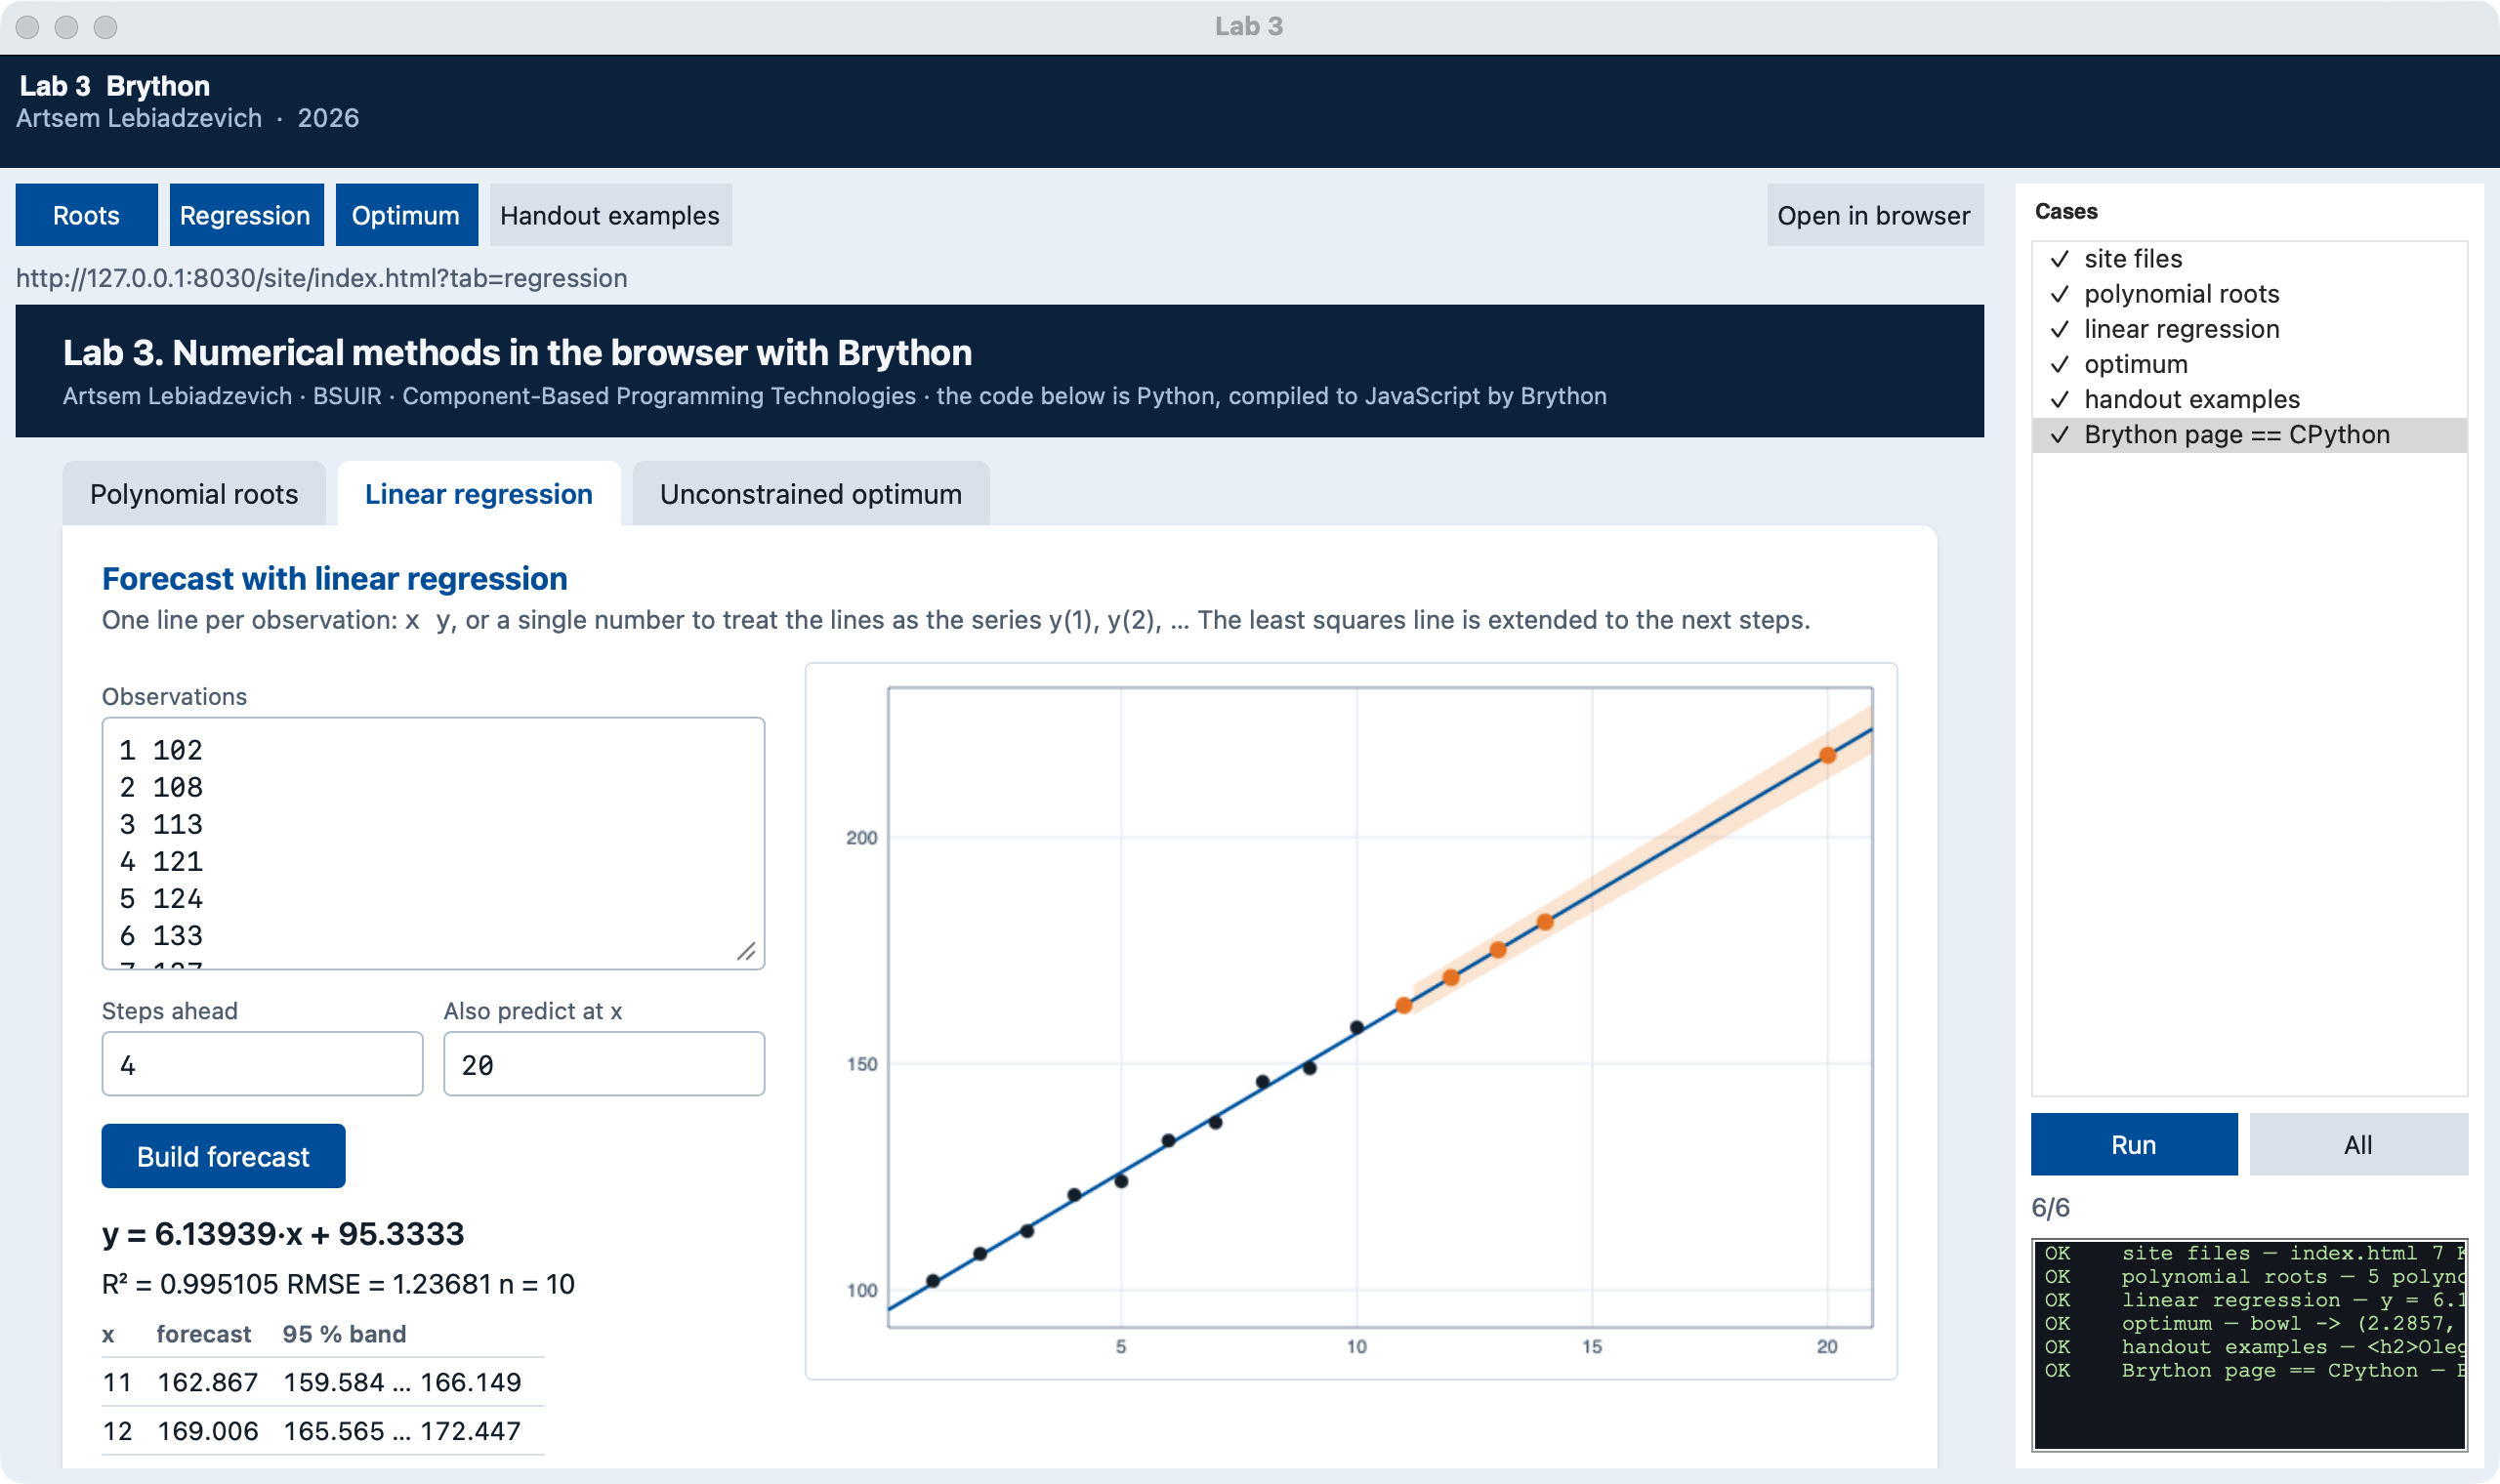
\includegraphics[width=0.95\textwidth]{../screenshots/lab3_regression.png}
\caption{Прогноз линейной регрессии}
\label{fig:reg}
\end{figure}

На рисунке~\ref{fig:opt} найден минимум функции $(x-1)^2+2(y+2)^2+xy$ методом Нелдера
--- Мида. Аналитическое решение системы $2(x-1)+y=0$, $4(y+2)+x=0$ даёт точку
$(16/7,\,-18/7)\approx(2{,}2857;\,-2{,}5714)$, она совпадает с найденной за 65 итераций.

\begin{figure}[H]
\centering
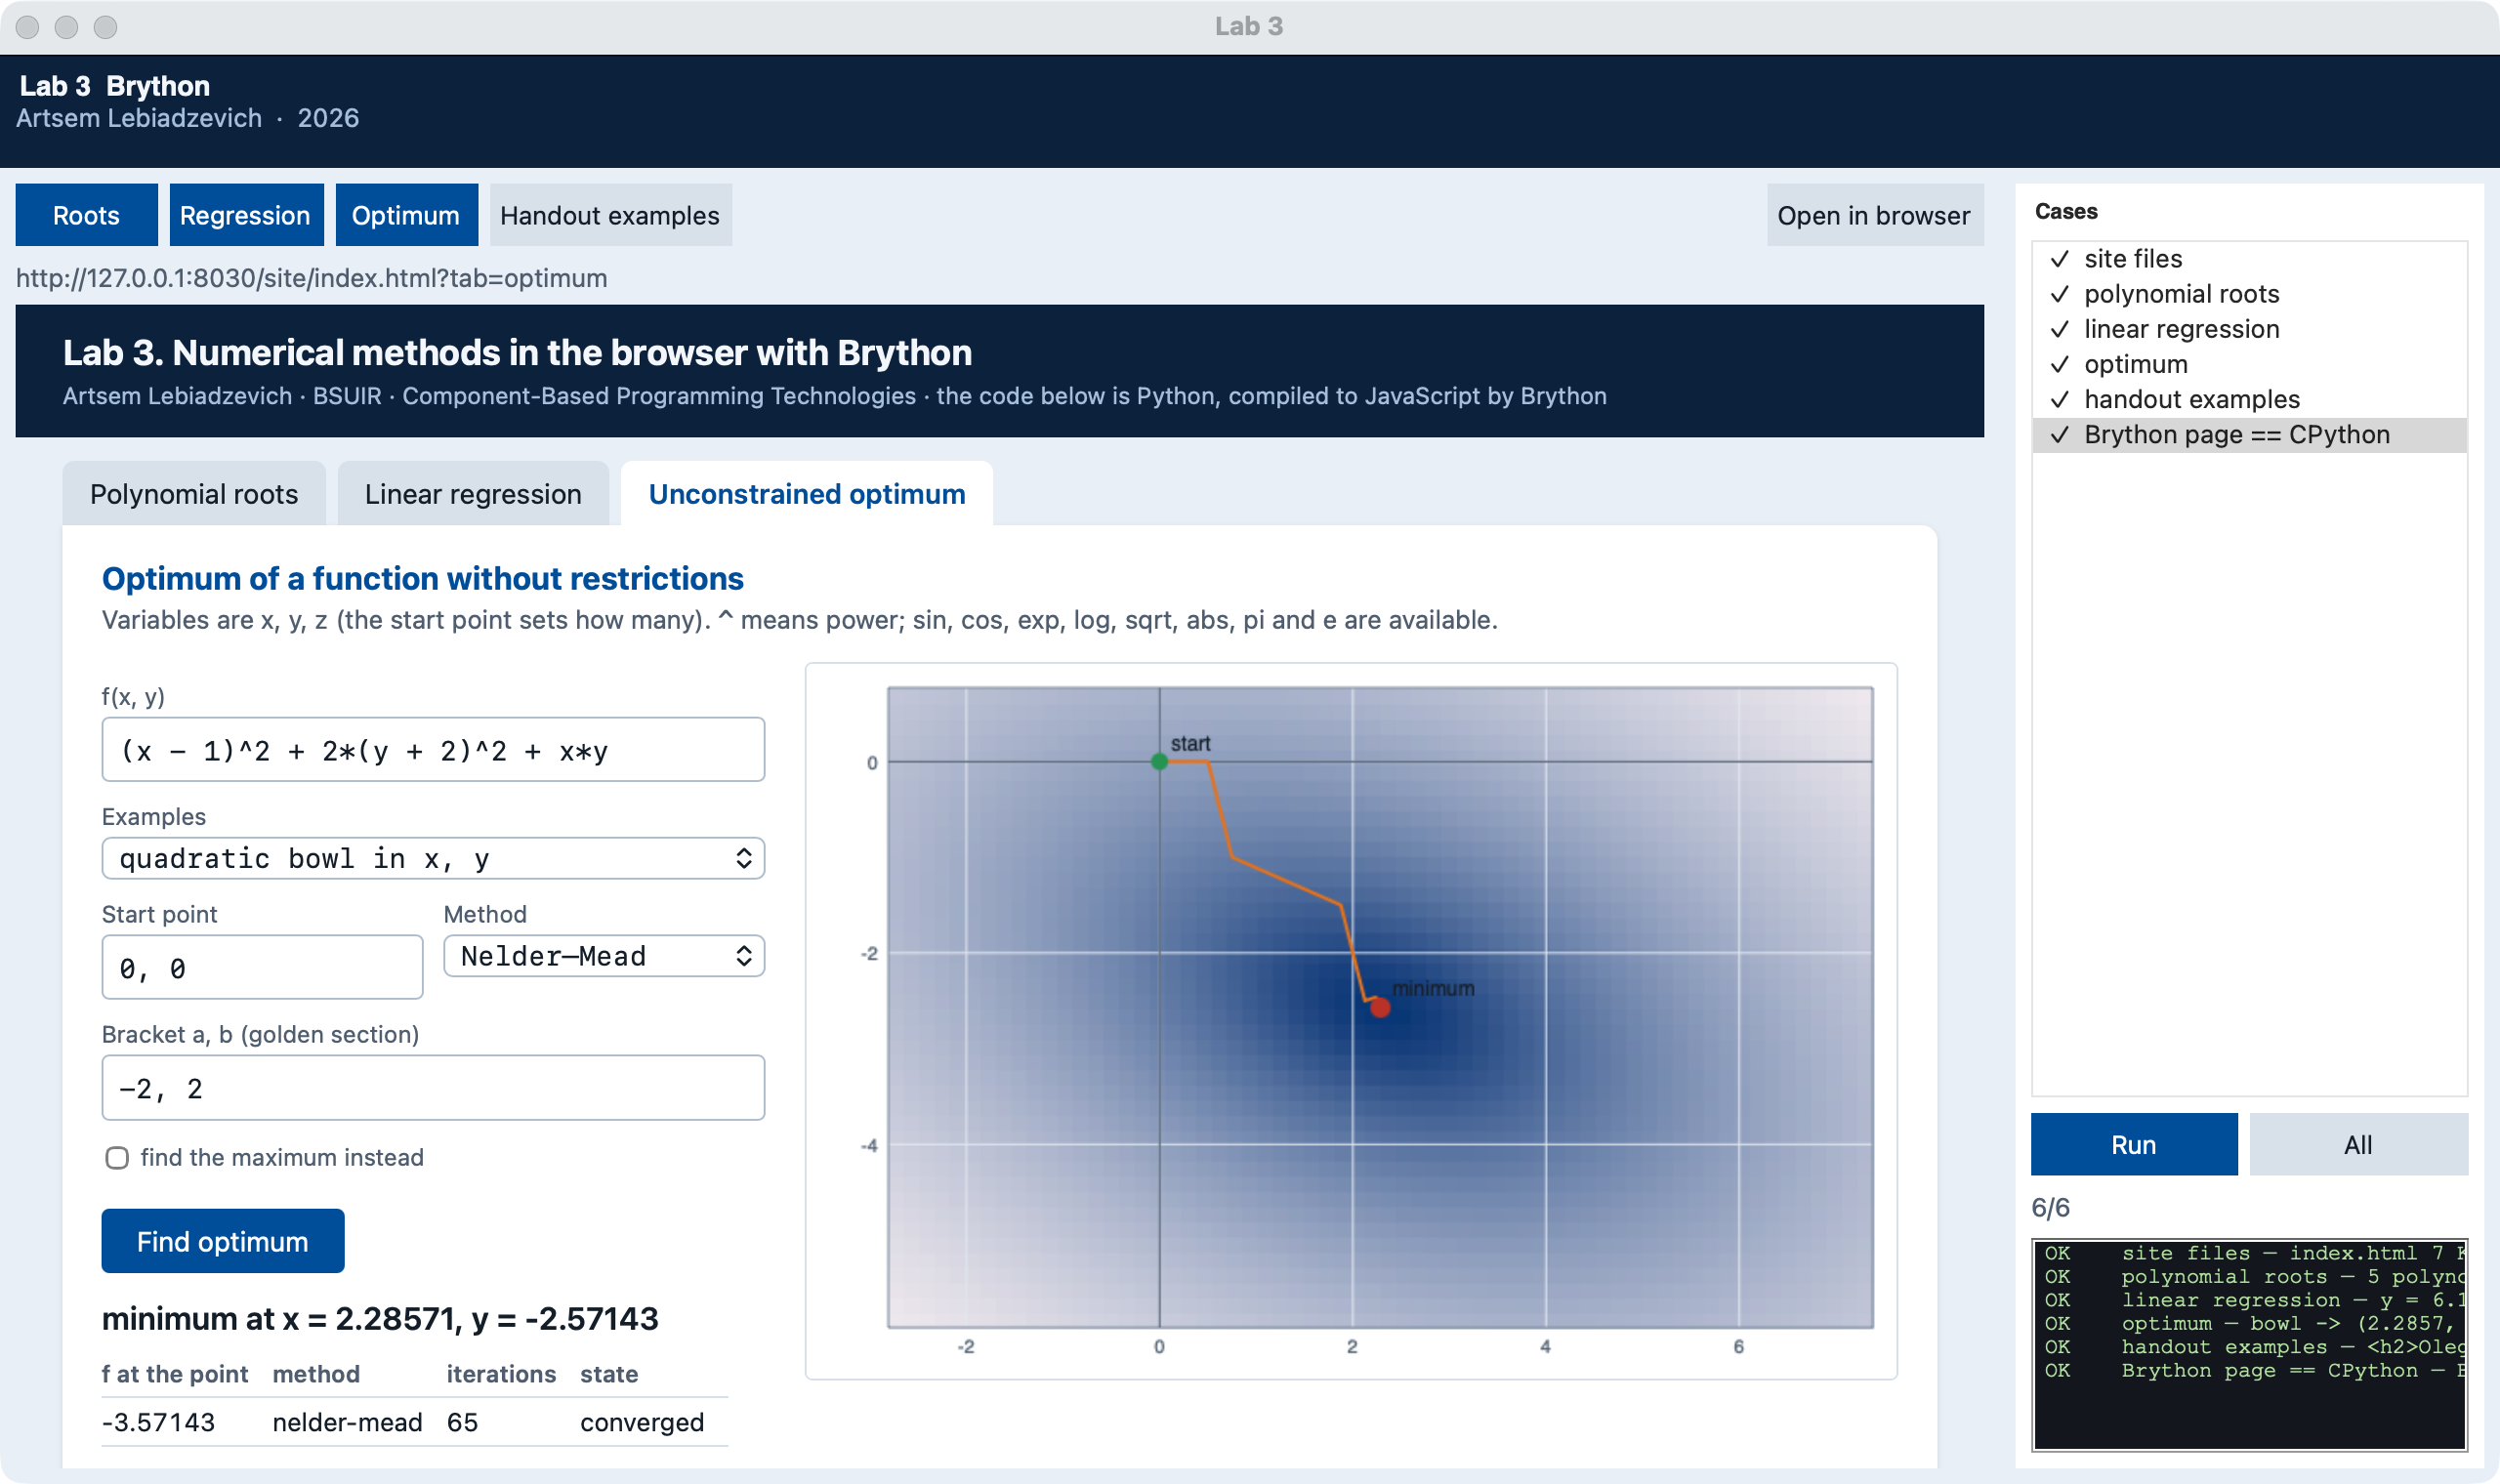
\includegraphics[width=0.95\textwidth]{../screenshots/lab3_optimum.png}
\caption{Минимум функции двух переменных: тепловая карта и траектория поиска}
\label{fig:opt}
\end{figure}

Примеры из методички (рисунок~\ref{fig:examples}) выполняются без изменений, кроме
явного \texttt{import browser.html}.

\begin{figure}[H]
\centering
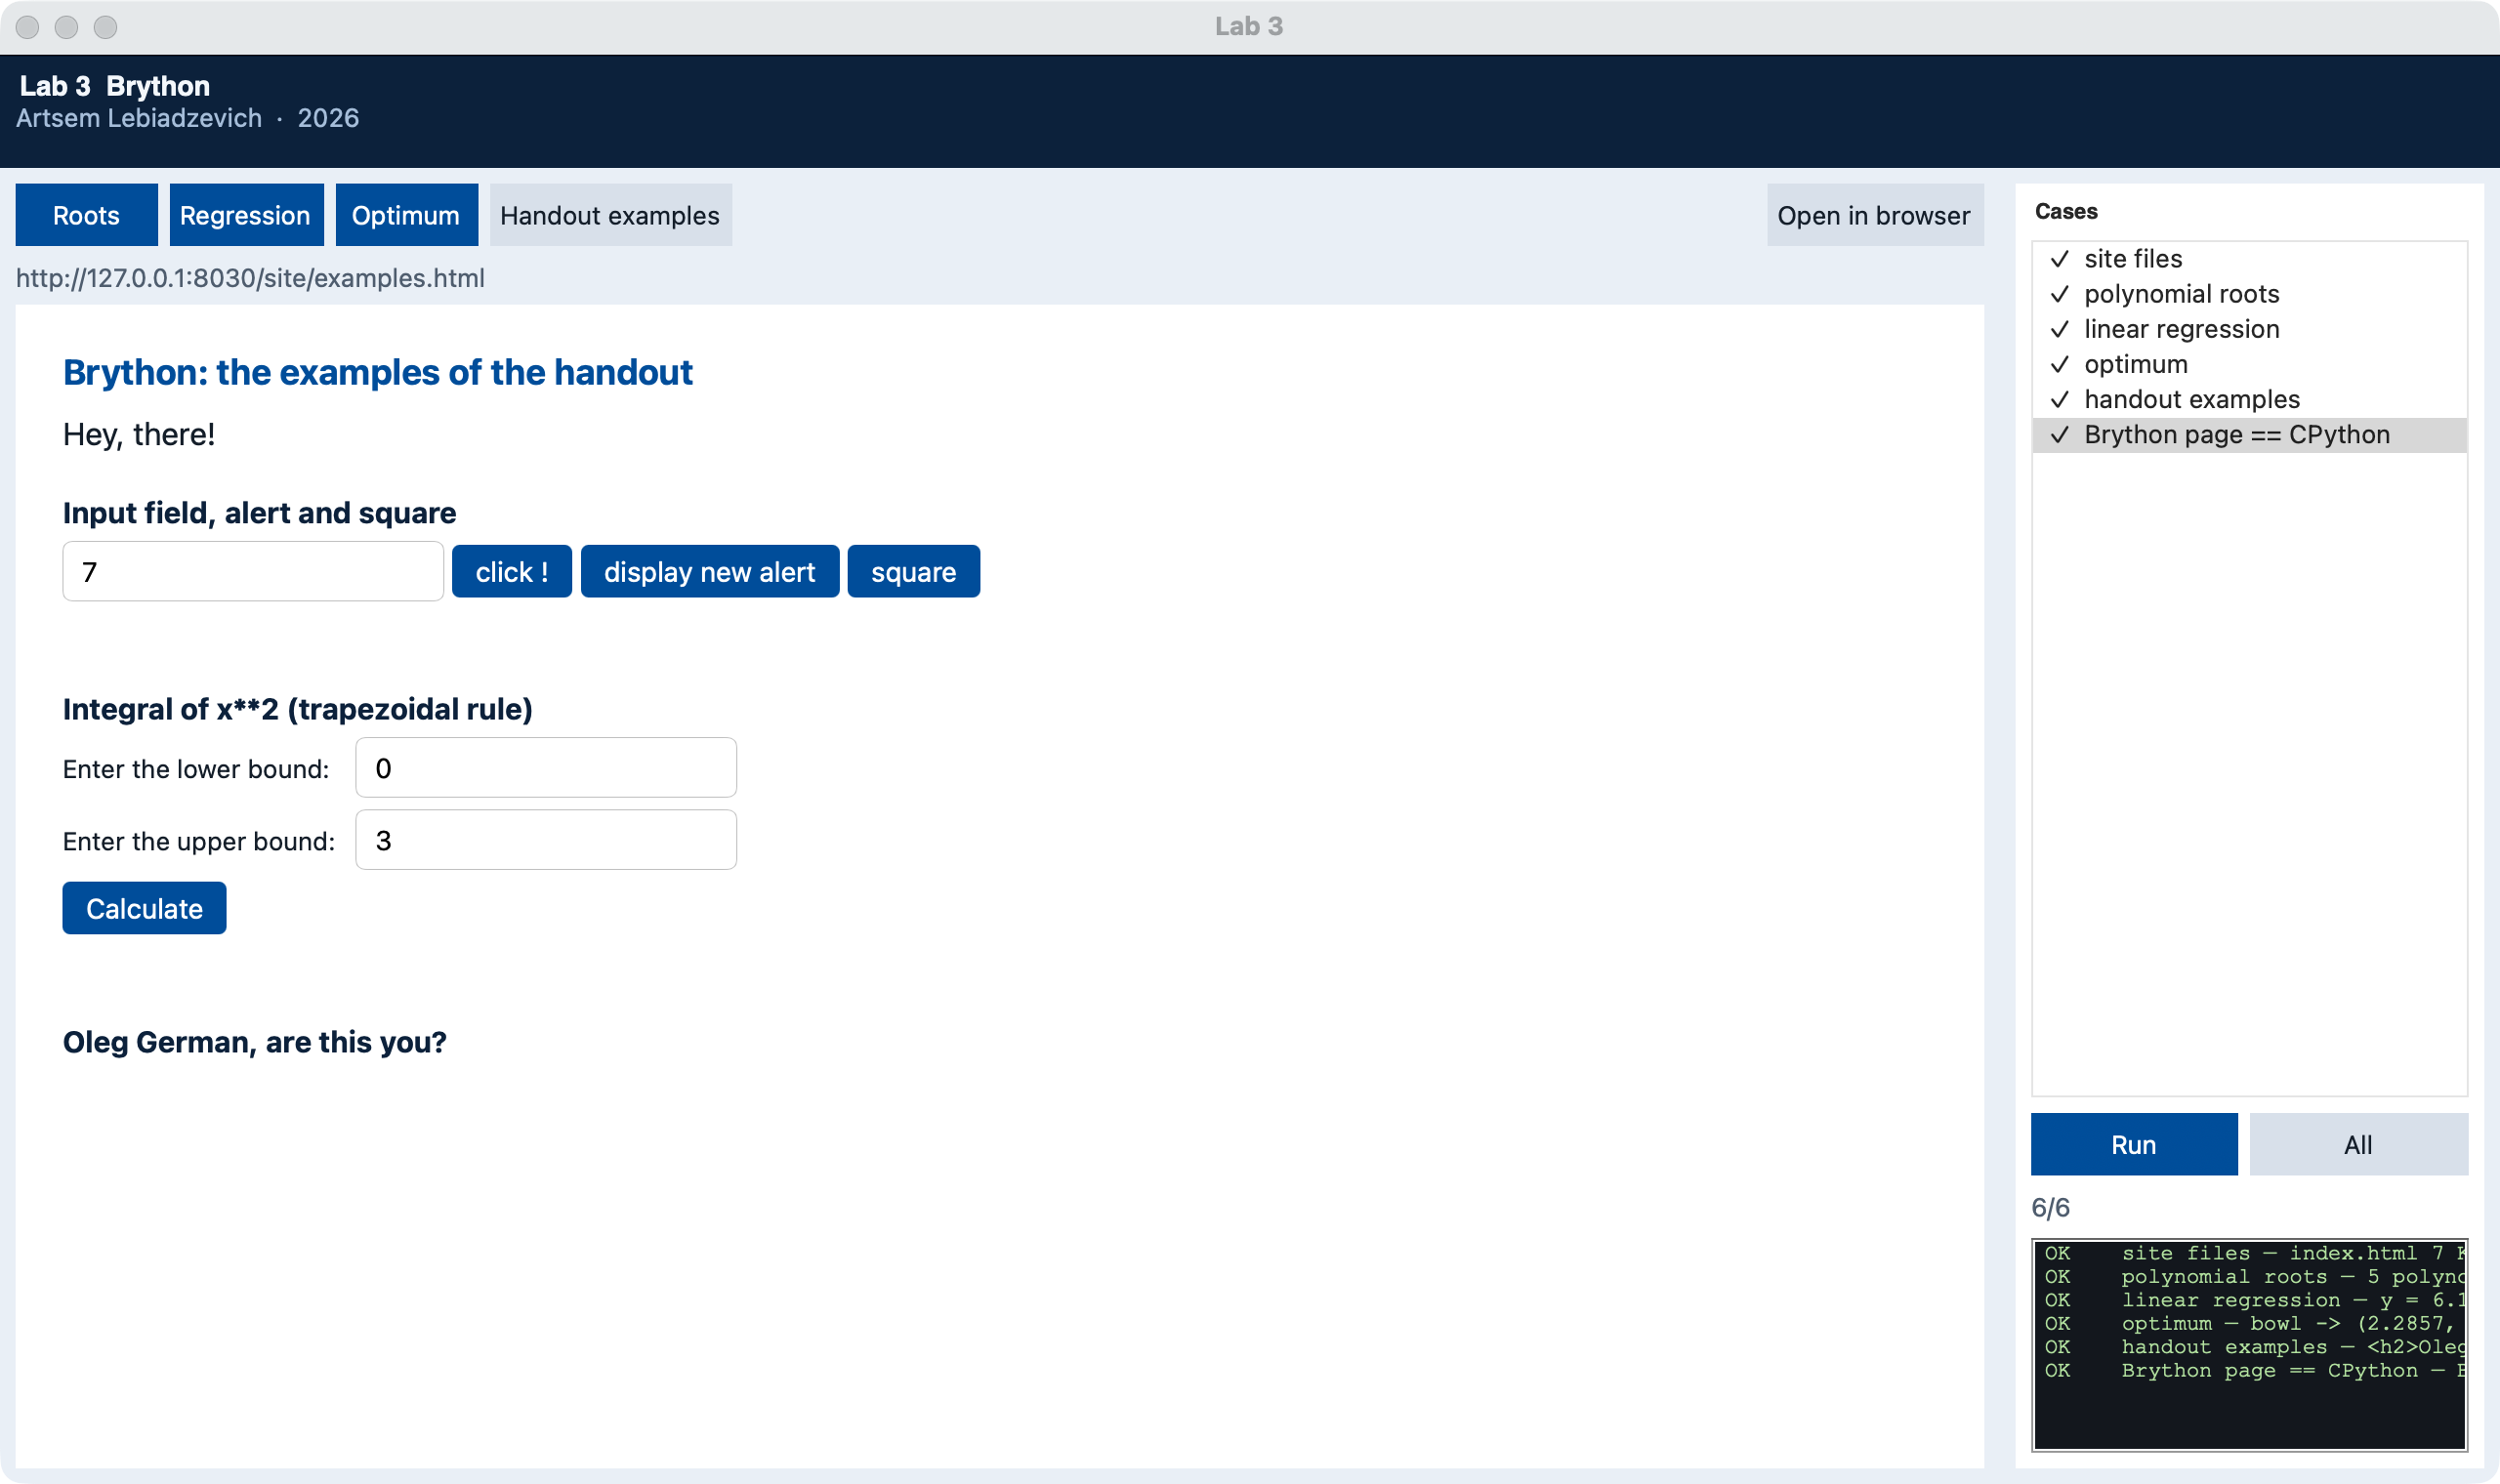
\includegraphics[width=0.95\textwidth]{../screenshots/lab3_examples.png}
\caption{Примеры из методических материалов}
\label{fig:examples}
\end{figure}

Команда \texttt{python main.py -{}-lab 3} выполняет те же сценарии без окна. Её вывод
приведён в листинге~\ref{lst:cli}. Последняя строка --- главная проверка: браузер без
окна открывает страницу, Brython выполняет \texttt{app.py}, страница записывает
вычисленные значения в DOM, и тест сравнивает 26 значений с результатами CPython.

\lstinputlisting[style=plain, caption={Вывод программы}, label={lst:cli}]{listings/cli_output.txt}

Сводка по результатам приведена в таблице~\ref{tab:results}.

\begin{table}[H]
\caption{Проверка численных методов}
\label{tab:results}
\centering
\small
\begin{tabularx}{\textwidth}{lLL}
\toprule
Задача & Исходные данные & Результат \\
\midrule
корни & $x^3-6x^2+11x-6$ & 1, 2, 3 \\
корни & $x^2+1$ & $-i$, $i$ \\
корни & $x^4-1$ & $-1$, $-i$, $i$, 1 \\
корни & $2x^4-8x^2$ & $-2$, 0, 0, 2 \\
регрессия & 10 точек & $y=6{,}139x+95{,}33$, $R^2=0{,}995$; в точке 11 --- 162,87 \\
оптимум & квадратичная функция & $(2{,}2857;\,-2{,}5714)$, как в аналитическом решении \\
оптимум & функция Розенброка & Нелдер --- Мид: $(1;\,1)$ за 126 шагов; градиентный спуск
достигает лимита 20\,000 итераций \\
оптимум & $x^4-3x^2+x$ & локальный минимум $x\approx1{,}131$ (градиентный спуск и золотое
сечение) \\
максимум & $\sin x\,e^{-0{,}1x}$ & $x=\operatorname{arctg}10\approx1{,}4711$ \\
\bottomrule
\end{tabularx}
\end{table}

Кроме сценариев окна написаны автоматические тесты: корни, регрессия (сверяется с
\texttt{statistics.linear\_regression}), методы оптимизации, отказ от посторонних имён в
функции, раздача общего модуля сервером и сравнение результатов Brython и CPython.
Все тесты проходят.

\section{Ответы на контрольные вопросы}

\textbf{1. Как создать клиентский сайт с помощью Brython?} Подключить
\texttt{brython.js} и \texttt{brython\_stdlib.js}, вызвать \texttt{brython()} из
\texttt{<body onload>}, написать код в блоке \texttt{<script type="text/python">}
(внутри страницы или в файле \texttt{src="app.py"}). Элементы получают как
\texttt{document["id"]}, обработчики подключают методом \texttt{bind("click", f)},
результат выводят в \texttt{.text} или добавляют элементы оператором
\texttt{document <= html.TAG(...)}.

\textbf{2. Как подключить библиотеки Python в сценарии Brython?} Стандартные модули
подключаются обычным \texttt{import}: они берутся из \texttt{brython\_stdlib.js}.
Собственные модули --- это файлы \texttt{.py} на сервере; Brython загружает их при
импорте, а каталог поиска задаётся параметром \texttt{pythonpath}
(\texttt{brython(\{pythonpath: ['/']\})}). Скомпилированные пакеты, например numpy,
недоступны, поэтому вычисления написаны на чистом Python.

\textbf{3. Объясните решение лабораторной работы.} Численные методы собраны в модуле
\texttt{numerics.py}; \texttt{app.py} читает поля страницы, вызывает методы, строит
таблицы и рисует на холсте; \texttt{index.html} содержит разметку. Сервер отдаёт
браузеру тот же \texttt{numerics.py}, который используют тесты, а отдельный тест
проверяет, что числа, вычисленные в браузере, совпадают с вычисленными в CPython.

\sectioncenter{Заключение}

В ходе лабораторной работы изучен фреймворк Brython и создан клиентский сайт, который
находит корни многочлена, строит прогноз линейной регрессии и ищет оптимум функции без
ограничений тремя методами. Весь код страницы, включая обработку событий, построение
таблиц и рисование на холсте, написан на Python.

Главный практический вывод: Brython позволяет использовать один и тот же модуль в
браузере и в обычном Python, поэтому численный код можно проверить автоматическими
тестами на сервере, а затем выполнять у клиента без изменений. Ограничения подхода тоже
видны: недоступны скомпилированные библиотеки, при загрузке страницы компилируется
стандартная библиотека объёмом 5\,МБ, а поведение зависит от версии фреймворка ---
примеры методички для версии 3.9 потребовали правки для версии 3.15.

\sectioncenter{Список использованных источников}

\begin{enumerate}
\item Герман, О.~В. Использование сценариев Python в HTML-документах с Brython:
лекция и лабораторная работа по дисциплине <<Технологии компонентного
программирования>> / О.~В.~Герман. --- Минск: БГУИР, 2024.
\item Brython documentation [Электронный ресурс]. --- Режим доступа:
\url{https://brython.info/static_doc/en/intro.html}.
\item Press, W.~H. Numerical Recipes: The Art of Scientific Computing /
W.~H.~Press [et al.]. --- 3rd ed. --- Cambridge: Cambridge University Press, 2007. ---
1256~p.
\item Nelder, J.~A. A simplex method for function minimization / J.~A.~Nelder,
R.~Mead // The Computer Journal. --- 1965. --- Vol.~7, No.~4. --- P.~308--313.
\end{enumerate}

\end{document}
